\thispagestyle{cackithitoannone}
\pagestyle{cackithitoan}
\everymath{\color{cackithi}}
\graphicspath{{../cackithi/pic/}}
\begingroup
\AddToShipoutPicture*{\put(0,616){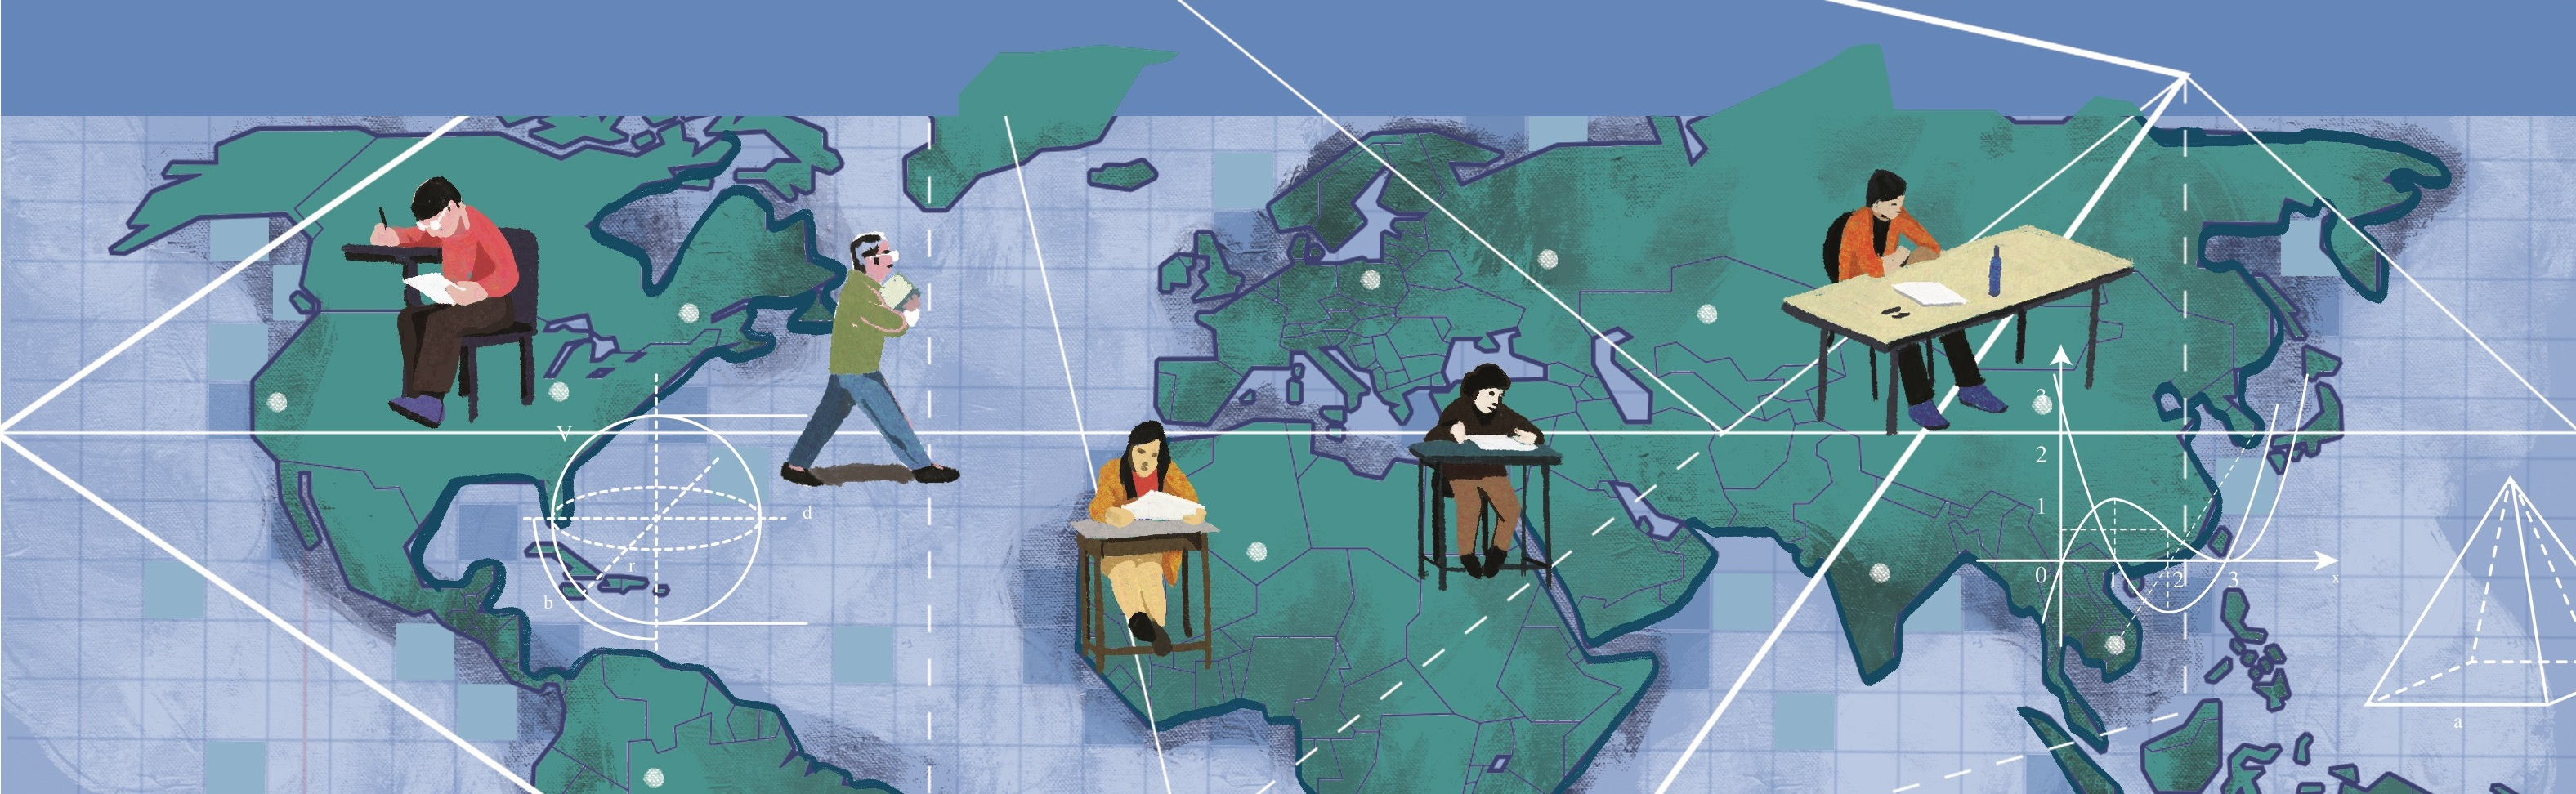
\includegraphics[width=19.3cm]{../bannercackithi}}}
\AddToShipoutPicture*{\put(150,572){
\includegraphics[scale=1]{../tieude1.pdf}}}
\centering
\endgroup
\vspace*{135pt}

\begin{multicols}{2}
	Trong phần đầu chuyên mục, chúng tôi sẽ trình bày với các bạn lời giải của các bài toán trong kỳ thi Olympic Toán học vùng Cáp--ca năm học $2022$ (Caucasus Math Olympiad), đăng trong số báo tháng $12/2022$. 
	\begin{figure}[H]
		\vspace*{-5pt}
		\centering
		\captionsetup{labelformat= empty, justification=centering}
		
\includegraphics[width= 1\linewidth]{gocolympic}
		\vspace*{-10pt}
	\end{figure}
	{\bf\color{cackithi} OC$\pmb{28.}$} Cho trước các số nguyên dương $a, b, c$. Biết rằng $\dfrac{c}{b} = \dfrac{b}{a}$, và $b^2 - a - c + 1$ là số nguyên tố. Chứng minh rằng $\dfrac{a}{2}$ và $\dfrac{c}{2}$ là các số chính phương.
	\vskip 0.1cm
	\textit{Lời giải.} Từ đầu bài ta có $b^2=ac,$ từ đó thu được  $b^2 - a - c + 1=(a-1)(c-1)$ là số nguyên tố. Như vậy một trong hai số $a$ hoặc $c$ phải bằng $2$. Không mất tổng quát, giả sử $a=2,$ khi đó $b^2=2c$ như vậy $b$ là chẵn. Đặt $b=2k,$ thì $c=2k^2.$ Như vậy ta có điều cần chứng minh: $\dfrac{a}{2}=1$ và $\dfrac{c}{2}=k^2.$
	\vskip 0.1cm
	{\bf\color{cackithi} OC$\pmb{29.}$} Cho hình bình hành $ABCD$, các điểm $E$ và $F$ lần lượt nằm trên các đoạn $AD$ và $CD$ sao cho $\angle BCE = \angle BAF$. Các điểm $K$ và $L$ lần lượt nằm trên các đoạn $AD$ và $CD$ sao cho $AK = ED$ và $CL = FD.$ Chứng minh rằng $\angle BKD = \angle BLD.$
	\begin{figure}[H]
		\vspace*{-5pt}
		\centering
		\captionsetup{labelformat= empty, justification=centering}
		\begin{tikzpicture}[cackithi]
			\draw [shift={(6,3)},fill=cackithi,fill opacity=0.10000000149011612] (0,0) -- (180:0.33403201021243345) arc (180:225:0.33403201021243345) -- cycle;
			\draw [shift={(0,0)},fill=cackithi,fill opacity=0.10000000149011612] (0,0) -- (11.309932474020219:0.33403201021243345) arc (11.309932474020219:56.309932474020215:0.33403201021243345) -- cycle;
			\draw  (0,0)-- (2,3);
			\draw  (2,3)-- (6,3);
			\draw  (6,3)-- (3,0);
			\draw  (0,0)-- (4.615384615384616,0.9230769230769236);
			\draw  (2,3)-- (5.384615384615384,2.0769230769230758);
			\draw  (0,0)-- (1,0);
			\draw  (0.5,0.10020960306372992) -- (0.5,-0.10020960306372992);
			\draw  (1,0)-- (3,0);
			\draw  (3,0)-- (4,0);
			\draw  (3.5,0.10020960306372992) -- (3.5,-0.10020960306372992);
			\draw  (4,0)-- (4.615384615384616,0.9230769230769236);
			\draw  (4.201151925266359,0.4823833189696255) -- (4.36791078471567,0.3712107460034184);
			\draw  (4.2474738306689455,0.5518661770735044) -- (4.414232690118257,0.44069360410729735);
			\draw  (4.615384615384616,0.9230769230769236)-- (5.384615384615384,2.0769230769230758);
			\draw  (5.384615384615384,2.0769230769230758)-- (6,3);
			\draw  (5.585767309881747,2.559306395892701) -- (5.752526169331055,2.4481338229264944);
			\draw  (5.632089215284331,2.6287892539965805) -- (5.79884807473364,2.5176166810303733);
				\draw [fill=white] (0,0) circle (1.5pt);
				\draw (-0.22221545793430705,-0.21615426902148865) node {$A$};
				\draw [fill=white] (2,3) circle (1.5pt);
				\draw (1.8988878069146455,3.4414962428046536) node {$B$};
				\draw [fill=white] (6,3) circle (1.5pt);
				\draw (6.141094336612552,3.357988240251545) node {$C$};
				\draw [fill=white] (4,0) circle (1.5pt);
				\draw (4.003289471252977,-0.28296067106397527) node {$D$};
				\draw [fill=white] (3,0) circle (1.5pt);
				\draw (2.9510886390838107,-0.2662590705533536) node {$E$};
				\draw [fill=white] (1,0) circle (1.5pt);
				\draw (0.9970013793410751,-0.249557470042732) node {$K$};
				\draw [fill=white] (4.615384615384616,0.9230769230769236) circle (1.5pt);
				\draw (4.888474298315926,0.9863609677432703) node {$F$};
				\draw [fill=white] (5.384615384615384,2.0769230769230758) circle (1.5pt);
				\draw (5.706852723336388,2.055263400423056) node {$L$};
		\end{tikzpicture}
		\vspace*{-5pt}
	\end{figure}
	\textit{Lời giải.}
	Từ giả thiết, ta có
	\begin{align*}
		\angle ECD&= \angle BCD - \angle BCE \\
		&= \angle BAD - \angle BAF = \angle FAD.
	\end{align*}
 %%%
	Ta thu được hai tam giác $ECF$ và $FAD$ đồng dạng và từ đó có đẳng thức $\dfrac{ED}{FD} = \dfrac{DC}{DA}.$ Mặt khác ta có $\dfrac{ED}{FD} = \dfrac{AK}{CL}$ và $\dfrac{DC}{DA}=\dfrac{AB}{CB}.$ Do đó ta nhận được $\dfrac{AK}{CL}=\dfrac{AB}{CB},$  suy ra hai tam giác $AKB$ và $CLB$ đồng dạng. 
	\vskip 0.1cm
	Như vậy, ta có $\angle AKB=\angle CLB$ do đó nhận được   $\angle BKD = \angle BLD.$
	\vskip 0.1cm
	{\bf\color{cackithi} OC$\pmb{30.}$} Peter viết ra $21$ số nguyên dương đôi một phân biệt, mỗi số không lớn hơn $10^6$. Đối với mỗi cặp số $(a, b)$ được Peter viết ra, Nick  viết  số
	\begin{align*}
		F(a, b) = a + b - \gcd (a, b)
	\end{align*}
	trên mảnh giấy của mình (ở đây $\gcd$ ký hiệu ước chung lớn nhất). 
	\vskip 0.1cm
	Chứng minh rằng một trong những số mà Nick viết khác với tất cả những  số mà Peter viết. 
	\vskip 0.1cm
	\textit{Lời giải.} Ta chứng minh bằng phản chứng. Giả sử mọi số mà Nick viết ra đều trùng với một trong các số mà Peter đã viết. Ta xếp các số Peter viết theo thứ tự tăng dần:
	\begin{align*}
		a_1 < a_2 < \cdots < a_{20} < a_{21}.
	\end{align*}
	Khi đó, do $\gcd (a_{20}, a_{21}) \le a_{20},$ ta có  $F(a_{20}, a_{21}) = a_{20} + a_{21} - \gcd (a_{20}, a_{21})\ge a_{21}.$ Như vậy dấu bằng phải xảy ra, tức là $\gcd (a_{20}, a_{21}) = a_{20}$ ta suy ra $a_{21}$ là bội của $a_{20}.$
	\vskip 0.1cm
	Ta sẽ chứng minh $a_{k+1}$ là bội của $a_k$ với mọi $k=1, \cdots, 20.$ Thật vậy, với $k=20$ điều này đúng. Giả sử trái lại, gọi $k<20$ là số lớn nhất mà $a_{k+1}$ không là bội của $a_k.$ Khi đó, lý luận như trên ta có $F(a_{k}, a_{k+1})>a_{k+1}$. Mặt khác, do $a_{k+2}$ là bội của $a_{k+1},$ ta có 
	\begin{align*}
		F(a_{k}, a_{k+1}) &= a_{k} + a_{k+1} - \gcd (a_{k}, a_{k+1})\\
		&<  a_{k} + a_{k+1}< 2a_{k+1}\le a_{k+2}.
	\end{align*}
	Như vậy $F(a_{k}, a_{k+1})$ không trùng với bất kỳ số nào Peter viết ra, điều này mâu thuẫn với giả thiết phản chứng. Vậy ta chứng minh được $a_{k+1}$ là bội của $a_k$ với mọi $k=1, \cdots, 20.$
	\vskip 0.1cm
	Từ đây ta có
	\begin{align*}
		a_{21}&\ge 2a_{20} \ge 2^2 a_{19} \ge \cdots \ge 2^{19}a_2 \ge 2^{20}a_1\\
		&\ge 2^{20}>10^6.
	\end{align*}
	Điều này trái với giả thiết, như vậy ta có điều cần chứng minh. 
	\vskip 0.1cm
	Trong phần cuối của chuyên mục kỳ này, chúng tôi sẽ giới thiệu với bạn đọc ba bài toán trong kỳ thi toán của Đan Mạch mang tên nhà toán học Georg Mohr. Các bài toán này phù hợp với trình độ học sinh lớp $5-7$.
	\vskip 0.1cm
	{\bf\color{cackithi} OC$\pmb{37.}$} Một con ếch nhảy vào các số nguyên trên trục số. Nếu đang ở một số $n$ chẵn, bước tiếp theo nó sẽ nhảy đến số $\dfrac{n}{2}.$ Nếu đang ở một $n$ số lẻ, nó sẽ nhảy đến số $n + 5$. Tại một thời điểm nó nhảy vào số $25$. Hỏi trước đó 3 bước nó có thể ở những vị trí nào?
	\vskip 0.1cm
	{\bf\color{cackithi} OC$\pmb{38.}$} Các số $1, 2, 3, \cdots, 16$  được đặt trong $16$ ô vuông xung quanh một bảng ô vuông cỡ $5\times 5$ như hình bên sao cho tổng của $5$ số trên mỗi cạnh của hình vuông là bằng nhau. 
	Tổng nhỏ nhất có thể có của bốn số trong các ô vuông ở góc là bao nhiêu?
	\begin{figure}[H]
		\vspace*{-5pt}
		\centering
		\captionsetup{labelformat= empty, justification=centering}
		\begin{tikzpicture}[scale=0.8,cackithi]
			\draw (0,0) grid (5,5);
			\draw[fill=white] (1,1) rectangle(4,4);
		\end{tikzpicture}
		\vspace*{-10pt}
	\end{figure}
	{\bf\color{cackithi} OC$\pmb{39.}$} Cho hình đa giác đều 9 cạnh $ABCDEFGHI$ như hình vẽ. Chứng minh rằng $AB + AC =AE.$
	\begin{figure}[H]
		\vspace*{-5pt}
		\centering
		\captionsetup{labelformat= empty, justification=centering}
		\begin{tikzpicture}[cackithi,scale=0.8]
			\draw  (1,2)-- (3,2);
			\draw  (3,2)-- (4.532088886237956,3.2855752193730785);
			\draw  (4.532088886237956,3.2855752193730785)-- (4.879385241571817,5.255190725397494);
			\draw  (4.879385241571817,5.255190725397494)-- (3.879385241571817,6.9872415329663715);
			\draw  (3.879385241571817,6.9872415329663715)-- (2,7.671281819617709);
			\draw  (2,7.671281819617709)-- (0.12061475842818448,6.987241532966372);
			\draw  (0.12061475842818448,6.987241532966372)-- (-0.8793852415718164,5.255190725397496);
			\draw  (-0.8793852415718164,5.255190725397496)-- (-0.5320888862379562,3.28557521937308);
			\draw  (-0.5320888862379562,3.28557521937308)-- (1,2);
			\draw  (1,2)-- (4.532088886237956,3.2855752193730785);
			\draw  (1,2)-- (3.879385241571817,6.9872415329663715);
				\draw [fill=white] (1,2) circle (1.5pt);
				\draw (0.7965821732136155,1.687828189189382) node {$A$};
				\draw [fill=white] (3,2) circle (1.5pt);
				\draw (3.1515078452112713,1.7212313902106253) node {$B$};
				\draw [fill=white] (4.532088886237956,3.2855752193730785) circle (1.5pt);
				\draw (4.855071097294682,3.2744802376984405) node {$C$};
				\draw [fill=white] (4.879385241571817,5.255190725397494) circle (1.5pt);
				\draw (5.222506308528359,5.4122851030580135) node {$D$};
				\draw [fill=white] (3.879385241571817,6.9872415329663715) circle (1.5pt);
				\draw (4.019991071763599,7.349670762290128) node {$E$};
				\draw [fill=white] (2,7.671281819617709) circle (1.5pt);
				\draw (2.0157990104889976,8.18475078782121) node {$F$};
				\draw [fill=white] (0.12061475842818448,6.987241532966372) circle (1.5pt);
				\draw (-0.13870745538119822,7.383073963311371) node {$G$};
				\draw [fill=white] (-0.8793852415718164,5.255190725397496) circle (1.5pt);
				\draw (-1.2243114885716069,5.345478701015527) node {$H$};
				\draw [fill=white] (-0.5320888862379562,3.28557521937308) circle (1.5pt);
				\draw (-0.7566666742742002,3.040657830549737) node {$I$};
		\end{tikzpicture}
		\vspace*{-5pt}
	\end{figure}
\end{multicols}